\documentclass[a4paper, 10pt, twocolumn, twoside]{article}

\usepackage{main}
\usepackage{amsmath}

\usepackage[linesnumbered]{algorithm2e}
\SetKwComment{Comment}{/* }{ */}
\newtheorem{theorem}{Theorem}
\usepackage{siunitx}
\usepackage{lscape}
\usepackage{hologo}
\usepackage{listings}

\usepackage{pgfplots}
 
\pgfplotsset{compat = newest}

% Table stretch
\usepackage{array}
\usepackage{xcolor}
\lstset { %
    language=C++,
    backgroundcolor=\color{black!5}, % set backgroundcolor
    basicstyle=\footnotesize,% basic font setting
}

\begin{document}

 % Do not change the following line
\linespread{0.5}

\title{Expected weight of the minimum spanning trees\\ of Euclidean and random complete graphs}

\author{Swati Goel$^{1}$ and Lev Kruglyak$^2$}

% \affiliation{
% $^1$Harvard University\\
% $^2$Harvard Univertity
% }

\email{
\href{mailto:e.sgoel@college.harvard.edu}{sgoel@college.harvard.edu$^1$}, 
\href{mailto:e.levkruglyak@college.harvard.edu}{levkruglyak@college.harvard.edu$^2$}
}

% Do not change the following three lines
\maketitle 
\thispagestyle{fancy} 
\pagestyle{fancy}

\section{Introduction}
\label{sec:Introduction}

In this report, we would like to experimentally determine the asymptotic behavior of the average total weight of a minimum spanning tree of some random graphs as the number of vertices becomes very large. Specifically, we consider the following two types of graphs:
\begin{itemize}
    \item \textbf{Random Complete Graphs:} A complete undirected graph on $n$ vertices where the weight of each edge $(u,v)$ is chosen randomly and uniformly from the real interval $[0,1]$.
    \item \textbf{Random Euclidean Graphs:} (EG) A complete undirected graph on $n$ vertices in the unit hypercube $[0,1]^d$, where the weight of an edge $(u,v)$ is the Euclidean distance $\|u-v\|$. 
\end{itemize}

For the sake of generality, we'll refer to a random complete graph as a $0$-dimensional EG. Since the $1$-dimensional case isn't very interesting, we are thus interested in the $0$-dimensional case (i.e. just a random complete graph), and the $2,3,4$-dimensional cases. Let $f_d(n)$ be the expected total weight of a random $d$-dimensional Euclidean graph. (Including the $0$-dimensional case). Our goal is then to find an asymptotic expansion of $f_d(n)$.
\section{Random complete graphs}

The naive approach to computing the MST of a random complete graph would be to simply build up the graph in its entirety and then run an MST algorithm on the generated graph, which may be optimized for very dense graphs. Using something like Prim's algorithm with a Fibonacci heap, we could get a runtime of $O(V^2+V\log V)$ where $V$ is the number of vertices in the graph. This turns out to be highly unfeasible since it requires storing $V^2$ edges, which can easily surpass the maximum memory of any reasonable computer. There are a few ways to get around this limitation.

\subsection{Procedural random graphs}
\label{sec:Preparation}

Using procedural random functions we can actually dispense with storing the graph at all, reducing the space complexity to constant. As opposed to an iterative random function which outputs a sequence of random numbers based on the order in which it was called, a procedural random function takes in some input, and consistently returns the same random number every time it is called. 

So a procedural random graph need only contain the number of verticies in the graph and a seed value. The graph comes with some procedural random function which takes in a seed and two edge indices. (We can pick the random function so that it is symmetric in the edge indicies, so that the graph is property undirected) Then every time we want to fetch an edge, we simply call this procedural random function, and it will return the same random edge weight. Such procedural random functions can be easily created by composing several cryptographic integer functions and then using some bit manipulations to convert this to a float.

To find the MST of such a procedural graph, we apply Prim's algorithm to this graph interface, since Prim's algorithm does not require any storing of edges. In practice, we found that this approach was too slow, so we switched to a different approach.

\subsection{Sparsifying a random complete graph}

A secondary approach to this problem is to build a sparse graph on $n$ vertices, by only adding edges to the graph when the weight of the edge is less than some threshold $\kappa(n)$. Ideally, this bound would be chosen not to change the minimum spanning tree. For our implementation, we experimentally determined that an upper bound of the form
\[
    \kappa(n)=c\frac{\log_2 n}{n}
\]
works, where $c$ is some fixed constant. We deduced the value of $c$ by starting it at some very high number so the generated graph would be complete, any slowly lowering it until the weight of the minimum spanning tree changes significantly. We found that a $c$-value of approximately $c\approx 4.0$ seems to work.

We then run Kruskal's algorithm on this reduced graph, giving us a minimum spanning tree. Assuming a uniformly distributed random function, the number of edges is $O(\kappa(n)\cdot n^2)=O(n\log n)$. Thus the time complexity of Kruskal's algorithm applied to this sparse graph is $O(n\log^2 n)$. This is a more reasonable time frame. 

\subsection{Numerical results}

For each $n$, we ran $8$ trials, each in a separate thread for maximum performance, and then the results were averaged. Computing all these values took about 30 minutes on a 2.3 GHz 8-Core Intel Core i9 Macbook Pro
with 16 GB 2667 MHz DDR4 memory, which was fairly expected based on the algorithm's performance for smaller values and the asymptotic time complexity.

\renewcommand{\arraystretch}{1.5}
\begin{table}[htbp]
\centering
\caption{Random complete graph MST weights}
\begin{tabular}{||c|c||c|c||}
\hline
$n$ & $f_0(n)$ & $n$ & $f_0(n)$ \\
\hline
$2^7$ &1.10562 & $2^{13}$  &1.21397\\
$2^8$	&1.09412 & $2^{14}$  &1.2037\\
$2^9$&1.0523 &$2^{15}$  &1.21013\\
$2^{10}$ &1.15964 &$2^{16}$  &1.2026\\
$2^{11}$  &1.16696 & $2^{17}$  &1.20162\\
$2^{12}$  &1.17769 & $2^{18}$  &1.20655\\
\hline
\end{tabular}
\end{table}

The asymptotic expansion of $f_0(n)$ appears to be constant, converging to $\lim_{n\to \infty} f_0(n)\approx 1.206$. This is somewhat intuitively understandable, since given any node $u$, we can on average find an edge to some node $v$ with weight approximately equal to $1 /n$. Then the MST should have about $n$ nodes and so the total weight is some constant factor.

\subsection{Theoretical asymptotic expansion for $f_{0}(n)$}

There already exists a theoretical limit for the expected weight of a random complete graph, somewhat surprisingly it is related to the Riemann zeta function from analytic number theory. See \cite{Fr1985} for a proof.

\begin{theorem}
    Given a complete graph on $n$ verticies, where the edge weights are uniformly distributed in the $[0,1]$ interval, the expected weight of an MST of this graph approaches the constant $\zeta(3)$ as $n\to \infty$ where $\zeta(s)$ is the Riemann zeta function:
    \[
        \zeta(s)=\sum^\infty_{k=0}\frac{1}{k^s}
    \]
    The constant $\zeta(3)$ is known as Apéry's constant.
\end{theorem}

This theoretical result is inline with our experimental result, since
\[
    \zeta(3)=1.202\;056\;903\ldots
\]  
In dimensions $d\geq 2$, the asymptotics of $f_d(n)$ look very different, however there is much more optimization to be had in these Euclidean cases.

\section{Random Euclidean Graphs}

As opposed to a totally random complete graph, the edge weights on a Euclidean graphs have significantly more structure, which can lend itself to some incredible optimizations. For our implementation, we used the algorithm presented in \cite{SD2016}. 

This algorithm doesn't give an exact MST but an approximate one. More formally, given some point set $P\subset \mathbb{R}^d$ and error parameter $\varepsilon > 0$, the algorithm produces a Euclidean spanning tree for $P$ whose weight is at most $(1+\varepsilon)$ times the weight of the true minimum spanning tree. The algorithm does this with time complexity $O\left(n\log n + \left(\varepsilon^{-2}\log^2 \frac{1}{\varepsilon}\right)n\right)$. This algorithm is incredibly efficient and also quite simple.

\subsection{Overview of the algorithm}

\RestyleAlgo{ruled}
\begin{algorithm}
\caption{Approx-EMST($P, \varepsilon$)}
\DontPrintSemicolon
$Q(P) \leftarrow $ a quadtree for $P$\;
$\Psi(P)$ a $s$-WSPD for $P$\;
$G\leftarrow(P,\emptyset)$ 
 
% \SetKwFunction{shovel}{shovel}
% \SetKwProg{myalg}{procedure}{}{}

% \myalg{\shovel{$u,v\in V$}} {
%     assuming Pat is at $u$, shovel the sidewalk from $u$ to $v$.\;
%     Pat should now be at $v$.
% }\;

% \SetKwFunction{recursiveShovel}{recursive\_shovel}

% $\forall (i,j)\in E, e[i,j]\leftarrow 0$ \Comment*[r]{start all edges as not shovelled}
% \myalg{\recursiveShovel{$G(V,E), s\in V$}}{
%     \For(){$(s,v)\in E$}{
%         \If(){$e[s,v] = 0$ or $e[v,s]=0$}{
%             $e[s,v], e[v,s]\leftarrow 1$\Comment*[r]{mark edge as shovelled} 
%             \shovel{$s,v$}\Comment*[r]{point A}
%             \recursiveShovel{$G, v$}\;
%             \shovel{$v,s$}\Comment*[r]{point B}
%         }
%     }
% }
\end{algorithm}


\subsection{Numerical results}
As before, for each $n$ we ran $8$ trials, multithreaded for maximum performance and averaged the results. The algorithm ran very quickly; for a benchmark, it was able to calculate $f_4(2^{18})$ in under $20$ seconds. Letting the algorithm run for only a few minutes, we were able to obtain the following values:

\renewcommand{\arraystretch}{1.5}
\begin{table}[htbp]
\centering
\caption{Random Euclidean graph MST weights}
\begin{tabular}{||c|c|c|c||}
\hline
$n$ & $f_2(n)$ & $f_3(n)$ & $f_4(n)$ \\
\hline
$2^{7}$& 8.0888&	18.4344&	29.008\\
$2^{8}$&11.607& 29.234& 49.9654\\
$2^{9}$&16.5037&	46.3574&	83.9279\\
$2^{10}$&23.4344&	73.5039&	141.87\\
$2^{11}$&33.169& 116.624& 236.841\\
$2^{12}$&46.9872&	186.252&	401.888\\
$2^{13}$&66.5872&	293.833&	676.886\\
$2^{14}$&94.2845&	467.511&	1132.79\\
$2^{15}$&133.569& 742.982&	1898.65\\
$2^{16}$&188.905&	1177.78&	3223.1\\
$2^{17}$&267.479&	1872.09&	5415.15\\
$2^{18}$&378.2& 2969.83& 9060.04\\
$2^{19}$&534.991&	4713.59&	15187.7\\
$2^{20}$&756.245&	7484.55&	25787\\
\hline
\end{tabular}
\end{table}

If we plot these data points on a log-log graph (see Figure~\ref{fig}), we see that the data becomes almost perfectly linear, so we can run a linear regression to get an asymptotic approximation for $f_d(n)$. We then have the following asymptotic expessions for $f_d(n)$: $f_2(n)\in\Theta(n^{0.503})$, $f_3(n)\in \Theta(n^{0.667})$ and $f_4(n)\in \Theta(n^{0.752})$. This leads to the conjecture that for $d\geq 2$, $f_d(n)\in \Theta(n^{(d-1)/d})$. 

\subsection{Theoretical asymptotic expansion for $f_d(n)$}
In \cite{St1988}, an asymptotic expression for $f_d(n)$ is given in terms of the density of the probability distribution for picking points in the unit hypercube.

\begin{theorem}
    Let $f$ be the density of the probability function for picking points in the hypercube. Then for any $d>1$, the expected weight of the Euclidean minimum spanning tree approaches 
    \[
        c(d)n^{\frac{d-1}{d}}\int_{\mathbb{R}^d}f(x)^{\frac{d-1}{d}}dx
    \] 
    as $n\to \infty$. 
\end{theorem}

In particular, for a uniform probability distribution we have $f_d(n)\in \Theta(n^{\frac{d-1}{d}})$, confirming our conjecture.



\begin{figure}[htbp]
        \caption{log-log graph of $f_d(n)$ for $d=2,3,4$}
    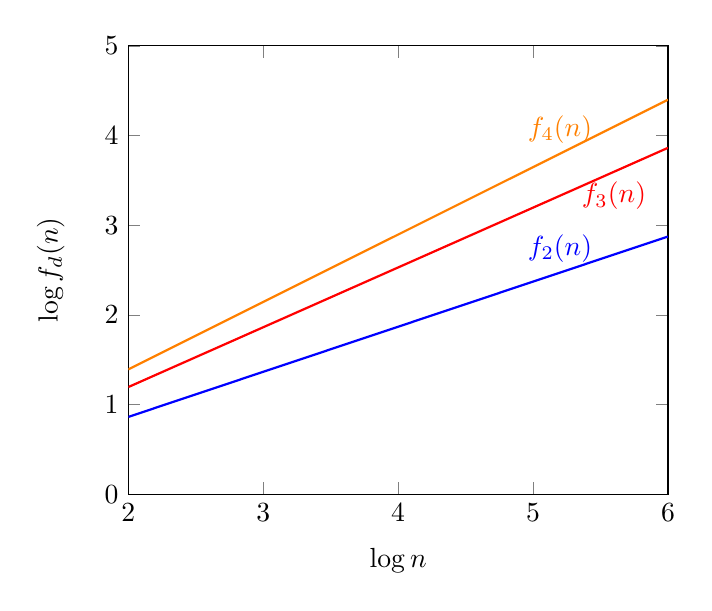
\begin{tikzpicture}
        \begin{axis}[
            xmin = 2, xmax = 6,
            ymin = 0, ymax = 5,
            x label style={at={(axis description cs:0.5,-0.1)},anchor=north},
            y label style={at={(axis description cs:-0.1,.5)},anchor=south},
            xlabel={$\log n$},
            ylabel={$\log f_d(n)$}]
            \addplot[
                domain = 2:6,
                samples = 200,
                smooth,
                thick,
                blue,
            ] {0.503*x-0.145} node[above,pos=0.8] {$f_2(n)$};;
            \addplot[
                domain = 2:6,
                samples = 200,
                smooth,
                thick,
                red,
            ] {0.667*x-0.14} node[below,pos=0.9] {$f_3(n)$};;
            \addplot[
                domain = 2:6,
                samples = 200,
                smooth,
                thick,
                orange,
            ] {0.752*x-0.113} node[above,pos=0.8] {$f_4(n)$};;
        \end{axis}
         
    \end{tikzpicture}
    \label{fig}
\end{figure}

\section{Conclusion}
\label{sec:Conclusion}

We thank you for considering using this \hologo{LaTeX} template for preparing your ISARC paper. 
Using \hologo{LaTeX} helps producing manuscripts that are formatted correctly first time, and thus avoid rework to you and the editorial team. 

If you have any question about the template and its guidelines, do not hesitate to contact the ISARC conference team.


\bibliography{main}

\end{document}
